% Template for ICASSP-2013 paper; to be used with:
%          spconf.sty  - ICASSP/ICIP LaTeX style file, and
%          IEEEbib.bst - IEEE bibliography style file.
% --------------------------------------------------------------------------
\documentclass{article}
\usepackage{spconf,amsmath,graphicx}
\usepackage{graphicx}
\usepackage{cite}
\usepackage{url}
% \usepackage{hyperref}
\usepackage{cleveref}
\usepackage{booktabs}
\usepackage{brian}

% Title.
% ------
\title{Learning to segment songs with ordinal linear discriminant analysis}
%
% Single address.
% ---------------
% \name{Author Names\thanks{Thanks to XYZ agency for funding.}}
% \address{Author Affiliations}
%
% For example:
% ------------
%\address{School\\
%   Department\\
%   Address}
%
% Two addresses (uncomment and modify for two-address case).
% ----------------------------------------------------------
\twoauthors%
 {Brian McFee\thanks{This work was supported by a grant from the Mellon foundation, and
grant IIS-1117015 from the National Science Foundation (NSF).}}{ Center for Jazz Studies\\
      Columbia University\\
  \texttt{brm2132@columbia.edu}}%
 {Daniel P.W. Ellis}{
  LabROSA, Department of Electrical Engineering\\
      Columbia University\\
  \texttt{dpwe@columbia.edu}}
%
\begin{document}
%\ninept
%
\maketitle
%
\begin{abstract}
This paper describes a supervised learning algorithm which optimizes a feature representation for temporally constrained clustering. 
The proposed method is applied to music segmentation, in which a song is partitioned into functional or
locally homogeneous segments (\eg, verse or chorus).  
To facilitate abstraction over multiple training examples, we develop a latent structural repetition feature, which summarizes the
repetitive structure of a song of any length in a fixed-dimensional representation.
Experimental results demonstrate that the proposed method efficiently integrates heterogeneous features, and improves segmentation accuracy.
\end{abstract}
%
\begin{keywords}
Music, automatic segmentation, learning
\end{keywords}
%
\section{Introduction}
\label{sec:intro}
% TODO:   2013-10-26 15:42:39 by Brian McFee <brm2132@columbia.edu>
% what is segmentation?
% how does it usually work?
% what's the problem with usual approaches

Automatic music segmentation algorithms take as input the acoustic signal of a musical performance, and produce a temporal
partitioning of the performance into a small number of \emph{segments}.  Ideally, segments correspond to structurally
meaningful regions of the performance, such \emph{verse} or \emph{chorus}.

Common approaches to music segmentation attempt to detect repeated patterns of features (\eg, a repeating chord progression),
often by some form of clustering~\cite{levy2008structural} or novelty detection~\cite{serra2012unsupervised}.  Often, features
are manually tuned and optimized for a specific development set, and carry implicit assumptions about the nature of musical 
structure.  As a concrete example, features built to detect repeated chord progressions may work well for characterizing some 
genres (\eg, rock or pop), but fail for other styles (\eg, jazz or hip-hop) which may be structured around timbre rather than melody.

In this work, we propose a supervised learning algorithm to automatically adapt acoustic and structural features to the statistics
of a training set. Given a collection of songs with structural annotations, the algorithm finds an optimal linear transformation
of features to preserve and predict segment boundaries.

\subsection{Our contributions}
Our primary contribution in this work is the ordinal linear discriminant analysis (OLDA) technique to learn a 
feature transformation which is optimized for musical segmentation, or more generally, time-series clustering.
As a secondary contribution, we propose a latent structural repetition descriptor, which facilitates learning and
generalization across multiple examples.

\subsection{Related work}
\label{sec:related}

The segmentation algorithm we use is most similar to the constrained clustering method of Levy and
Sandler~\cite{levy2008structural}, which incorporated sequential consistency constraints to a hidden Markov model. 
The method proposed here is simpler, and uses a sequentially constrained agglomerative clustering algorithm to 
produce a hierarchical segmentation over the entire track.  
Because the segmentation is hierarchical, the number of segments need not be specified in advance.

The proposed latent repetition features are adapted from the work of Serr\`{a}
\etal~\cite{serra2012unsupervised}. While qualitatively similar, we apply different filtering and
beat synchronization techniques to better preserve segment boundaries. 
In addition to chord sequence repetitions, our method includes timbre repetitions, as well as 
localized timbre, pitch, and timing information.

\section{Music segmentation}
\label{sec:features}
The criteria for deciding what is or is not a segment may vary across genres or styles.  
Pop music relies heavily on a verse/chorus structure, and is well characterized by repeating chord sequences. 
On the other hand, jazz tends to be structured by changing instrumentation (\eg, the current soloist),
and is better modeled as sequences of consistent timbre.
In general, a structural segmentation algorithm should include multiple feature representations in order to function
on various musical genres.

As a first step toward integrating multiple features, we introduce a structural repetition feature
which is amenable to learning and abstraction across multiple example songs.

\subsection{Latent structural repetition}
\Cref{fig:rep} outlines our approach for computing structural repetition features, which is adapted from
Serr\`{a} \etal~\cite{serra2012unsupervised}.  First, we extract beat-synchronous features (\eg, MFCCs or chroma) 
from the signal, and build a binary self-similarity matrix by linking each beat to its nearest neighbors in feature
space (\cref{fig:rep}, top-left).
Serr\`{a}~\etal{} incorporate local historical context by concatenating features from successive frames ${x_t \mapsto [x_t\trans, x_{t-1}\trans]\trans}$ prior 
to computing the self-similarity matrix.  We adopt this strategy, with the distinction that $x_{t}$ and $x_{t-1}$ are beat-synchronous.

With beat-synchronous features, repeated sections appear as diagonals in the self-similarity
matrix. To detect repeated sections, the matrix is skewed by shifting the $i$th column down by $i$ rows
(\cref{fig:rep}, top-right), thereby converting diagonals into horizontals.

Nearest-neighbor linkage can result spurious links and skipped connections. 
Serr\`{a}~\etal{} resolve this by convolving with a Gaussian filter, which suppresses noise, but also blurs
segment boundaries. Instead, we use a horizontal median filter, which (for odd window length) produces a binary matrix,
suppresses links outside of repeated sequences, and fills in skipped connections (\cref{fig:rep},
bottom-left).  The width of the median filter directly corresponds to the minimal duration (in beats) of detected repetitions,
and is consequently easier to tune than a Gaussian filter.
The median filter also preserves edges better than the Gaussian filter, so we may expect more precise detection of segment boundaries.

Let $R \in \R^{2t \times t}$ denote the median-filtered, skewed self-similarity matrix over $t$ beats.  
% Because different songs have different durations, the dimensionality of $R$ varies. 
Because the dimensionality (number of rows) of $R$ varies from one track to the next,
% This makes 
it is difficult to model and generalize across collections.
However, what matters for segmentation is not the representation of the columns of $R$, but the similarity between them.
More precisely, methods which depend on distances between column-vectors --- \ie, those based on clustering or novelty curves --- 
are invariant to unitary transformations $U\trans$:
$
\|R_{\cdot, i} - R_{\cdot, j}\| = \|U\trans R_{\cdot, i} - U\trans R_{\cdot, j}\|.
$ 

% Rather than use $R$ directly, 
We therefore introduce \emph{latent structural repetition}, which compresses each
any song's $R$ matrix to a fixed-dimension representation.  Let $R = U\Sigma V\trans$ denote the singular value decomposition of $R$,
with (descending) singular values $\sigma_i$. 
The latent structural repetition feature is defined as the matrix $L$:
\begin{equation}
L \defeq \sigma_1^{-1} U\trans R = \sigma_1^{-1} \Sigma V\trans.\label{eq:latent-rep}
\end{equation}

Reducing $L$ to $d < 2t$ principal components retains the most important factors, and normalizing by $\sigma_1$ reduces 
the influence of track duration. 
\Cref{fig:rep} (bottom-right) depicts an example of the resulting features.  
Small values of $d$ often suffice to capture global structure: in the given
example, the top component suffices to detect transitions between verse 
(non-repetitive) and chorus (repetitive).

\begin{figure}
\centering%
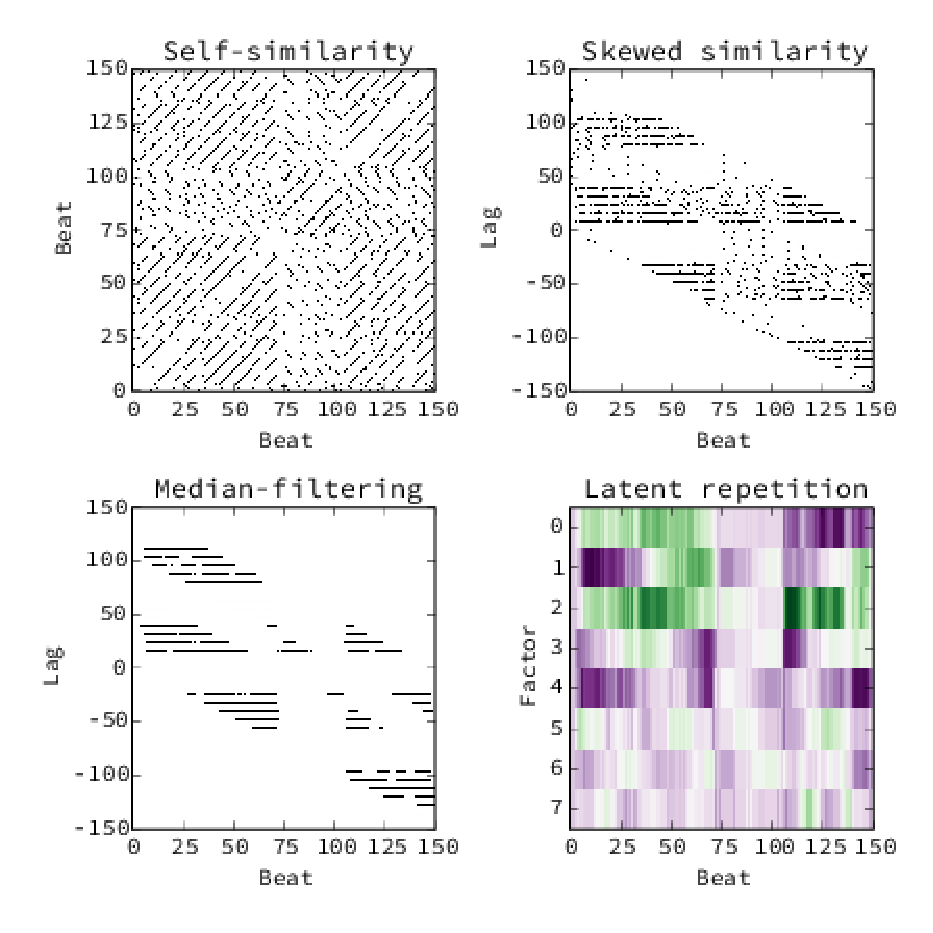
\includegraphics[width=\columnwidth]{figs/rep}
\vspace{-2\baselineskip}
\caption{Repetition features derived from \emph{Tupac Shakur --- Trapped}. 
Top-left: a binary self-similarity ($k$-nearest-neighbor) matrix over beats.
Top-right: the time-lag transformation of the self-similarity matrix.
Bottom-left: the result of the horizontal median filter.
Bottom-right: 8-dimensional latent factor representation (best viewed in color).}
\label{fig:rep}
\end{figure}

\subsection{Constrained agglomerative clustering}
\label{sec:clustering}
Given a feature matrix $X \in \R^{D\times t}$, we produce a hierarchical clustering of the columns of $X$ by using the
linkage-constrained variant of Ward's agglomerative clustering algorithm~\cite{ward1963hierarchical} as implemented in
\texttt{scikit-learn}~\cite{pedregosa2011scikit}.  For each column $X_{\cdot,i}$, linkage constraints are generated
for $(i-1, i)$ and $(i, i+1)$.  Starting from $t$ clusters (one for each column of $X$), 
linked clusters are iteratively merged until only one remains.
The hierarchy is computed in $\Oh(t)$ merge operations, and due to the constraints, 
there are $\Oh(t)$ feasible merges at each step. 
Each merge operation takes time $\Oh(D + \log t)$ (to compute centroids and manage a priority queue), so the algorithm runs in $\Oh(tD + t\log t)$ time.
For $D \in \Omega(\log t)$, the cost of clustering is dominated by the $\Omega(tD)$ cost of computing $X$.

\subsection{Choosing the number of segments}
The hierarchical clustering produces segmentations for all numbers of segments $1 \leq k \leq t$.  
Because music segmentation is itself an ambiguous task, the ability to simultaneously produce segmentations at all resolutions is a key advantage of the 
proposed technique.  
However, standard evaluation procedures are defined only for flat segmentations, and require a specific pruning of the segment hierarchy.

To select the number of segments $k$, we compute the clustering cost of each pruning within a plausible bounded range 
$k_{\min} \leq k \leq k_{\max}$.  The bounds are determined by assuming average minimum and maximum segment duration 
of 10s and 45s.  AIC correction~\cite{akaike1973information} is then applied to each candidate pruning (assuming a spherical 
Gaussian model for each segment), and $k$ is chosen to minimize the AIC-corrected cost.

\subsection{Multiple features}
Structural repetition features are most commonly used to detect repeated chord sequences, which is appropriate for
segmenting many genres of popular music.  However, the conventions of structure can vary from one genre to the next,
so a general segmentation algorithm should include a variety of feature descriptors.
We therefore aggregate several types of feature descriptors for each beat:
\begin{description}\addtolength{\itemsep}{-0.35\baselineskip}%
\item[Timbre] mean Mel-frequency cepstral coefficients,
\item[Pitch] (coordinate-wise) median chroma vectors,
\item[Timbre repetition] latent MFCC repetitions,
\item[Pitch repetition] latent chroma repetitions,
\item[Time] Time-stamp (in seconds) of each beat, normalized time-stamps (as a fraction of track duration), 
beat indices $(1, 2, \ldots, t)$, and normalized beat indices\\ $(1/t, 2/t, \ldots, 1)$.
\end{description}
Local timbre features can be useful for non-repetitive forms (\eg, jazz), while timbre repetition is useful for sample-based genres (\eg, hip-hop or electonic). 
Similarly, chroma features capture local pitch similarity, while pitch repetitions capture chord progressions.
The time features act as an implicit quadratic regularization on segment durations, and promote balanced segmentations. 
We include normalized and unnormalized time-stamps to allow the learning algorithm (\Cref{sec:olda}) to adapt the regularization to 
either relative or absolute segment durations; beat index features differ from raw time features by correcting for tempo variation.

All features can be stacked together into a single feature matrix $X \in \R^{D\times t}$, and clustered via the method described
above. However, the relative magnitude and importance of each feature is not calibrated to produce optimal clusterings. 

\section{Ordinal linear discriminant analysis}
%\begin{table*}
\centering
\caption{Segmentation performance. Best scores are indicated in bold; significance is assessed with a Bonferroni-corrected Wilcoxon
signed-rank test at $\alpha=0.05$.\label{tab:results}}
\footnotesize
\begin{tabular}{lrrrrrrrrrrrr}
% \bottomrule%
\multicolumn{13}{c}{Beatles-ISO}\\
\toprule%
Algorithm   &   $P_{0.5s}$ & $R_{0.5s}$ & $F_{0.5s}$ & $P_{3s}$     & $R_{3s}$  & $F_{3s}$   & $S_O$ & $S_U$ & $S_F$ & $P_C$& $R_C$& $F_C$\\
\hline
Unweighted  & 
0.274 & 0.218 & 0.237 & 0.606 & 0.469 & 0.518 & \textbf{0.842} & 0.755 & 0.791 & \textbf{0.780} & 0.613 & 0.668\\
FDA         &  
0.275 & 0.208 & 0.229 & 0.582 & 0.430 & 0.483 & \textbf{0.839} & 0.778 & 0.802 & \textbf{0.774} & 0.653 & 0.691\\
OLDA        & 
\textbf{0.299} & \textbf{0.296} & \textbf{0.289} & 0.601 & 0.577 & 0.573 & 0.828 & 0.808 & 0.813 & 0.744 & 0.686 & 0.694\\
\hline
SMGA~\hfill\cite{serra2012unsupervised} &  
0.147 & 0.172 & 0.156 & \textbf{0.627} & \textbf{0.728} & \textbf{0.661} & 0.811 & \textbf{0.858} & \textbf{0.829} & 0.702 &
\textbf{0.798} & \textbf{0.729}\\
\toprule%
\multicolumn{13}{c}{SALAMI-free}\\
\toprule%
Unweighted  & 
0.236 & 0.184 & 0.200 & 0.495 & 0.390 & 0.422 & 0.812 & 0.795 & 0.794 & 0.666 & 0.652 & 0.626\\
FDA     & 
\textbf{0.296} & 0.166 & 0.205 & \textbf{0.564} & 0.330 & 0.400 & 0.849 & 0.729 & 0.771 & 0.751 & 0.566 & 0.603\\
OLDA    & 
0.265 & \textbf{0.234} & \textbf{0.241} & 0.510 & 0.457 & 0.467 & 0.804 & 0.829 & \textbf{0.808} & 0.640 & 0.707 & \textbf{0.640}\\
\hline
SMGA~\hfill\cite{serra2012unsupervised} &
0.115 & 0.178 & 0.134 & 0.434 & \textbf{0.666} & \textbf{0.508} & 0.714 & \textbf{0.895} & 0.786 & 0.448 & \textbf{0.822} & 0.550\\
C-NMF~\hfill\cite{nieto2013convex}  &
0.105 & 0.133 & 0.110 & 0.450 & 0.543 & 0.463 & 0.767 & 0.797 & 0.767 & 0.576 & 0.639 & 0.550\\
SI-PLCA~\hfill\cite{weiss2011unsupervised}  &
0.210 & 0.102 & 0.128 & 0.451 & 0.228 & 0.286 & \textbf{0.873} & 0.538 & 0.643 & \textbf{0.814} & 0.362 & 0.459\\
\bottomrule%
\end{tabular}
\end{table*}


\label{sec:olda}
To improve the feature representation for clustering, we propose a simple adaptation of Fisher's linear discriminant
analysis (FDA)~\cite{fisher1936use}.  In its multi-class form, FDA takes as input a labeled collection of data $x_i \in \R^D$
and class labels $y_i \in \{1,2,\ldots, C\}$, and produces a linear transformation $W \in \R^{D\times D}$ that simultaneously 
maximizes the distance between class centroids, and minimizes the variance of each class 
individually~\cite{fukunaga1990introduction}. This is accomplished by solving the following optimization:
\begin{equation}
W \defeq \argmax_W \trace\left( {(W\trans A_\text{W} W)}^{-1} W\trans A_\text{B} W \right) \label{eq:fda},
\end{equation}
where $A_\text{W}$ and $A_\text{B}$ are the \emph{within-} and \emph{between}-class scatter matrices:
\begin{align*}
A_\text{W} & \defeq \sum_c \sum_{i : y_i = c} (x_i - \mu_c)(x_i - \mu_c)\trans\\
A_\text{B} & \defeq \sum_c n_c (\mu_c - \mu)(\mu_c - \mu)\trans,
\end{align*}
$\mu$ denotes the mean across all classes, $\mu_c$ is the mean of class $c$, and $n_c$ denotes the number of examples in class $c$.
\Cref{eq:fda} can be efficiently solved as a generalized eigenvalue problem over the two scatter matrices $(A_\text{B},
A_\text{W})$~\cite{de2005eigenproblems}.

Class labels can be synthesized from segments on an annotated training song, so that the columns of $X$ belonging to the first 
segment are assigned to class 1, the second segment to class 2, and so on.
However, interpreting each segment as a distinct class could result in a repeated verse being treated as two distinct classes which 
cannot be separated. 
A more serious problem with this formulation is that it is unclear how to generalize across multiple songs, as it would result in
FDA attempting to separate segments from different songs.%, which is somewhat meaningless for the single-song segmentation task.

Due to linkage constraints, the agglomerative clustering algorithm (\cref{sec:clustering}) only considers merge 
operations over successive segments $(c, c+1)$. This motivates a relaxed FDA formulation which only attempts to separate adjacent
segments.  This is accomplished by replacing the between-class scatter matrix $A_B$ with the resulting \emph{ordinal scatter matrix}:
\begin{align*}
A_\text{O} &\defeq \sum_{c < C} n_c (\mu_c - \mu_{c+}) (\mu_c - \mu_{c+})\trans\\
            &\phantom{\defeq \sum_{c < C}} + n_{c+1} (\mu_{c+1} - \mu_{c+}) (\mu_{c+1} - \mu_{c+})\trans\\
\mu_{c+} &\defeq \frac{n_c \mu_c + n_{c+1} \mu_{c+1} }{n_c + n_{c+1}}.
\end{align*}
Intuitively, $A_\text{O}$ measures the deviation of successive segments $(c, c+1)$ from their mutual centroid $\mu_{c+}$, 
which coincides with the comparison performed for merge operations in the agglomerative clustering algorithm.
Optimizing $W$ to maximize this deviation, while minimizing within-segment variance, should enhance the overall segmentation accuracy.  

To improve numerical stability when $A_\text{W}$ is singular, we include a smoothing parameter
$\lambda > 0$.\footnote{The same regularization strategy is applied to FDA in \Cref{sec:eval}.} 
The OLDA optimization takes the form:
\begin{equation}
W \defeq \argmax_W \trace\left( {(W\trans (A_\text{W} + \lambda I) W)}^{-1} W\trans A_\text{O} W \right) \label{eq:olda},
\end{equation}
which again can be solved efficiently as a generalized eigenvalue problem over the matrix pair 
$(A_\text{O}, A_\text{W} + \lambda I)$.

Because interactions are only measured between neighboring segments, it is 
straightforward to include data from multiple songs by summing their individual contributions to $A_\text{O}$ and $A_\text{W}$.
After learning $W$, the feature matrix $X$ for a previously unseen song is transformed via $X \mapsto W\trans X$, and then 
clustered as described in \Cref{sec:clustering}.

\section{Evaluation}
\label{sec:eval}
All proposed methods are implemented in Python with the \texttt{librosa} package.\footnote{Code is
available at \url{https://github.com/bmcfee/olda}.}  
All signals were downsampled to 22KHz mono, and analyzed with a 93ms window and 3ms hop.  MFCCs are generated from 128 Mel bands
with an 8KHz cutoff. We take 32 MFCCs and 12 log-magnitude chroma bins; repetition features are calculated with $2\sqrt{t}$ nearest neighbors 
under a standardized euclidean metric, median-filtered with a window of width 7, and reduced to 32 dimensions each.  
Including the four time-stamp features, the combined representation has dimension $D=112$. Beats were detected by the \emph{median-percussive} method~\cite{mcfee2014beat}.

\subsection{Data and metrics}
We evaluate predicted segmentations on two publicly available datasets:
\begin{description}\addtolength{\itemsep}{-0.25\baselineskip}%
\item[Beatles-ISO] 179 songs by the Beatles~\cite{harte2010towards,isophonicsbeatles}, and
\item[SALAMI-free] 253 songs from the SALAMI dataset~\cite{smith2011design} which are freely available on the 
Internet Archive~\cite{nieto2013convex}.
\end{description}
Both datasets provide labels for each annotated segment (\eg, \emph{verse} or \emph{chorus}), but we ignore these
labels in this set of experiments. Compared to the Beatles corpus, SALAMI consists of tracks by multiple artists, 
and has much more diversity of genre, style, and instrumentation.

On both datasets, we compare to SMGA~\cite{serra2012unsupervised}, which achieved the
highest performance in the 2012 MIREX structural segmentation evaluation~\cite{Downie2008}.
On SALAMI-Free, we include comparisons to C-NMF~\cite{nieto2013convex} and SI-PLCA~\cite{weiss2011unsupervised}.

For both datasets, we evaluate the unweighted feature representation (\emph{Native}), FDA optimization (using the
one-class-per-segment approach described in \Cref{sec:olda}), and OLDA.\@
To ensure fairness of evaluation, the FDA and OLDA models used on the Beatles-ISO were trained using only
SALAMI-free data, and vice versa.  FDA and OLDA were trained by optimizing $\lambda \in \{10^0, 10^1, \dots, 10^9\}$
to maximize $F_{0.5}$ score (see below) on the training set.

For each method and dataset, we report the precision, recall, and F-measure of boundary retrieval, using either a 0.5-second or 3-second window.\footnote{
For a detailed description of segmentation metrics, see~\cite{mirexstructure}.}


\subsection{Results}
\label{sec:results}
\begin{table}
\centering
\caption{Boundary detection accuracy. Best scores are indicated in bold; significance is assessed with a Bonferroni-corrected Wilcoxon signed-rank test at $\alpha=0.05$.\label{tab:results}}
\small
\begin{tabular}{lrrrrrr}
\multicolumn{7}{c}{Beatles-ISO}\\
\toprule%
Method & $P_{0.5}$       & $R_{0.5}$         & $F_{0.5}$         & $P_3$             & $R_3$             & $F_3$             \\
\hline
Native  & \textbf{0.307}    & 0.243             & 0.263             & 0.584             & 0.450             & 0.497             \\
FDA     & \textbf{0.304}    & \textbf{0.320}    & \textbf{0.300}    & 0.575             & 0.563             & 0.553             \\
OLDA    & \textbf{0.307}    & \textbf{0.326}    & \textbf{0.304}    & 0.574             & 0.562             & 0.551             \\
\hline
SMGA    & 0.144             & 0.169             & 0.153             & \textbf{0.621}    & \textbf{0.728}    & \textbf{0.658}    \\
\toprule%
\multicolumn{7}{c}{SALAMI-free}\\
\hline
Native  & 0.237             & 0.183             & 0.200             & \textbf{0.500}    & 0.394             & 0.427             \\
FDA     & \textbf{0.259}    & \textbf{0.232}    & \textbf{0.237}    & \textbf{0.500}    & 0.461             & 0.464             \\
OLDA    & \textbf{0.255}    & \textbf{0.240}    & \textbf{0.241}    & \textbf{0.497}    & 0.475             & 0.471             \\
\hline
SMGA    & 0.115             & 0.178             & 0.134             & 0.434             & \textbf{0.666}    & \textbf{0.508}    \\
CNMF    & 0.105             & 0.133             & 0.110             & 0.450             & 0.543             & 0.463             \\
SI-PLCA & 0.210             & 0.102             & 0.128             & 0.451             & 0.228             & 0.286             \\
\bottomrule%
\end{tabular}
\end{table}

% \begin{table}
\centering
\caption{Segmentation performance. Best scores are indicated in bold; significance is assessed with a Bonferroni-corrected Wilcoxon
signed-rank test at $\alpha=0.05$.\label{tab:results}}
% \footnotesize
\begin{tabular}{lrrrr}
% \bottomrule%
\multicolumn{5}{c}{Beatles-ISO}\\
\toprule%
Algorithm   & $F_{0.5s}$ & $F_{3s}$   & $S_F$ & $F_C$\\
\hline
Unweighted  & 0.237             & 0.518             & 0.791             & 0.668\\
FDA         & 0.229             & 0.483             & 0.802             & 0.691\\
OLDA        & \textbf{0.294}    & 0.573             & 0.812             & 0.694\\
\hline
SMGA~\hfill\cite{serra2012unsupervised} 
            & 0.156             & \textbf{0.661}    & \textbf{0.829}    & \textbf{0.729}\\
\toprule%
\multicolumn{5}{c}{SALAMI-free}\\
\toprule%
Unweighted  & 0.200             & 0.422             & 0.794             & 0.626\\
FDA         & \textbf{0.234}    & 0.466             & \textbf{0.807}    & \textbf{0.641}\\
OLDA        & \textbf{0.241}    & 0.470             & \textbf{0.808}    & \textbf{0.641}\\
\hline
SMGA~\hfill\cite{serra2012unsupervised} 
            & 0.134             & \textbf{0.508}    & 0.786             & 0.550\\
C-NMF~\hfill\cite{nieto2013convex}  
            & 0.110             & 0.463             & 0.767             & 0.550\\
SI-PLCA~\hfill\cite{weiss2011unsupervised}  
            & 0.128             & 0.286             & 0.643             & 0.459\\
\bottomrule%
\end{tabular}
\end{table}


\Cref{tab:results} lists the results for the Beatles-ISO and SALAMI-free.
SMGA achieves highest performance with a 3-second window on both datasets.\footnote{SMGA parameters were tuned to perform well on the Beatles data~\cite{serra2012unsupervised}.}\@
% The NCE scores are qualitatively comparable between SMGA and OLDA ($S_F$ of 0.829 and 0.812, respectively).
The proposed methods achieve higher accuracy for boundary detection at 0.5s resolution, which can be attributed to the increased
accuracy afforded by the beat-synchronous and median-filtered repetition features.  

FDA and OLDA consistently improve over the baseline (Native), and achieve comparable F-scores. 
However, the FDA method tends to improve precision at the expense of recall, which indicates a tendency toward under-segmentation.
The OLDA method is adapted to only distinguish successive segments, and exhibits better boundary recall.

\section{Conclusion}
\label{sec:conclusion}
This paper introduced the ordinal linear discriminant analysis (OLDA) method for learning feature projections to improve time-series clustering.
The proposed latent structural repetition features provide a convenient, fixed-dimensional representation of global song structure, which 
facilitates modeling across multiple songs.

\section{Acknowledgments}
The authors thank Oriol Nieto for discovering an evaluation error in an early draft of this work.
The authors acknowledge support from The Andrew W. Mellon Foundation, and NSF grant IIS-1117015.

\bibliographystyle{IEEEbib}
\bibliography{refs}

\end{document}
